\chapter{Interfejs graficzny}
\label{chapter:gui}

\begin{figure}[ht!]
  \centering
  \fbox{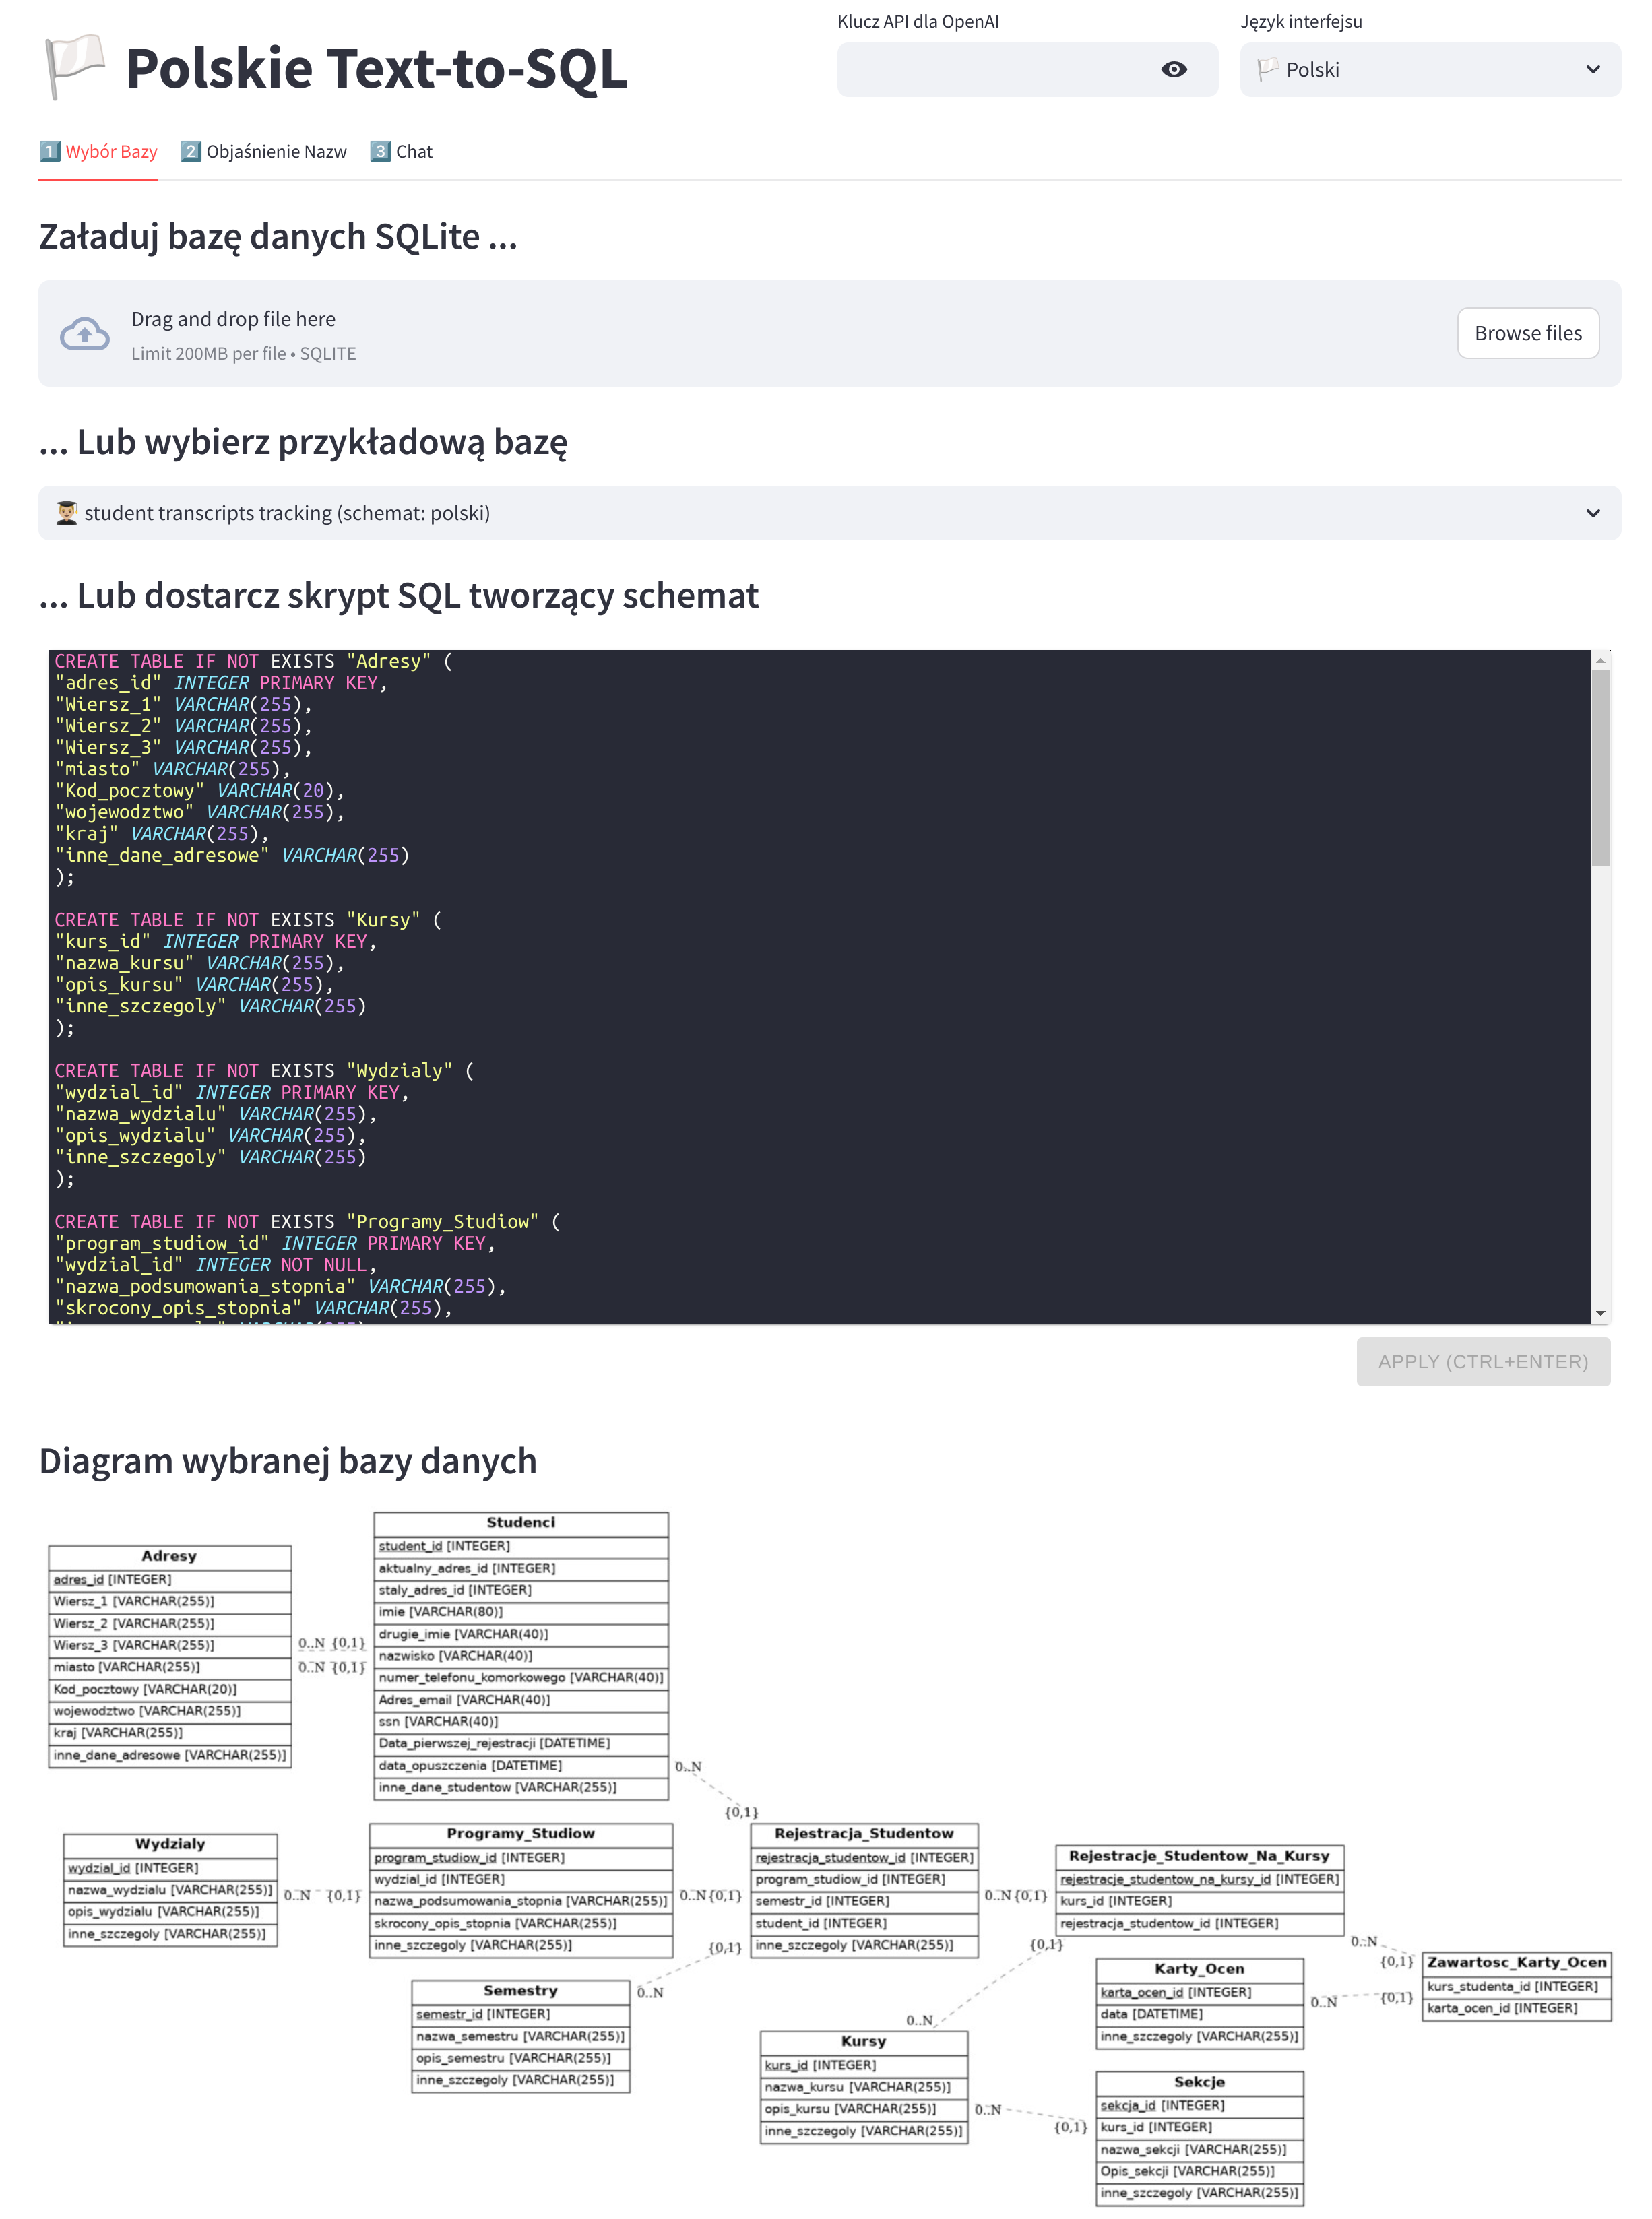
\includegraphics[width=1.0\linewidth]{images/gui_selection_tab.png}}
  \caption{Zakładka wyboru bazy danych w stworzonym interfejsie graficznym}
  \label{fig:gui-selection-tab}
\end{figure}

\begin{figure}[ht!]
  \centering
  \fbox{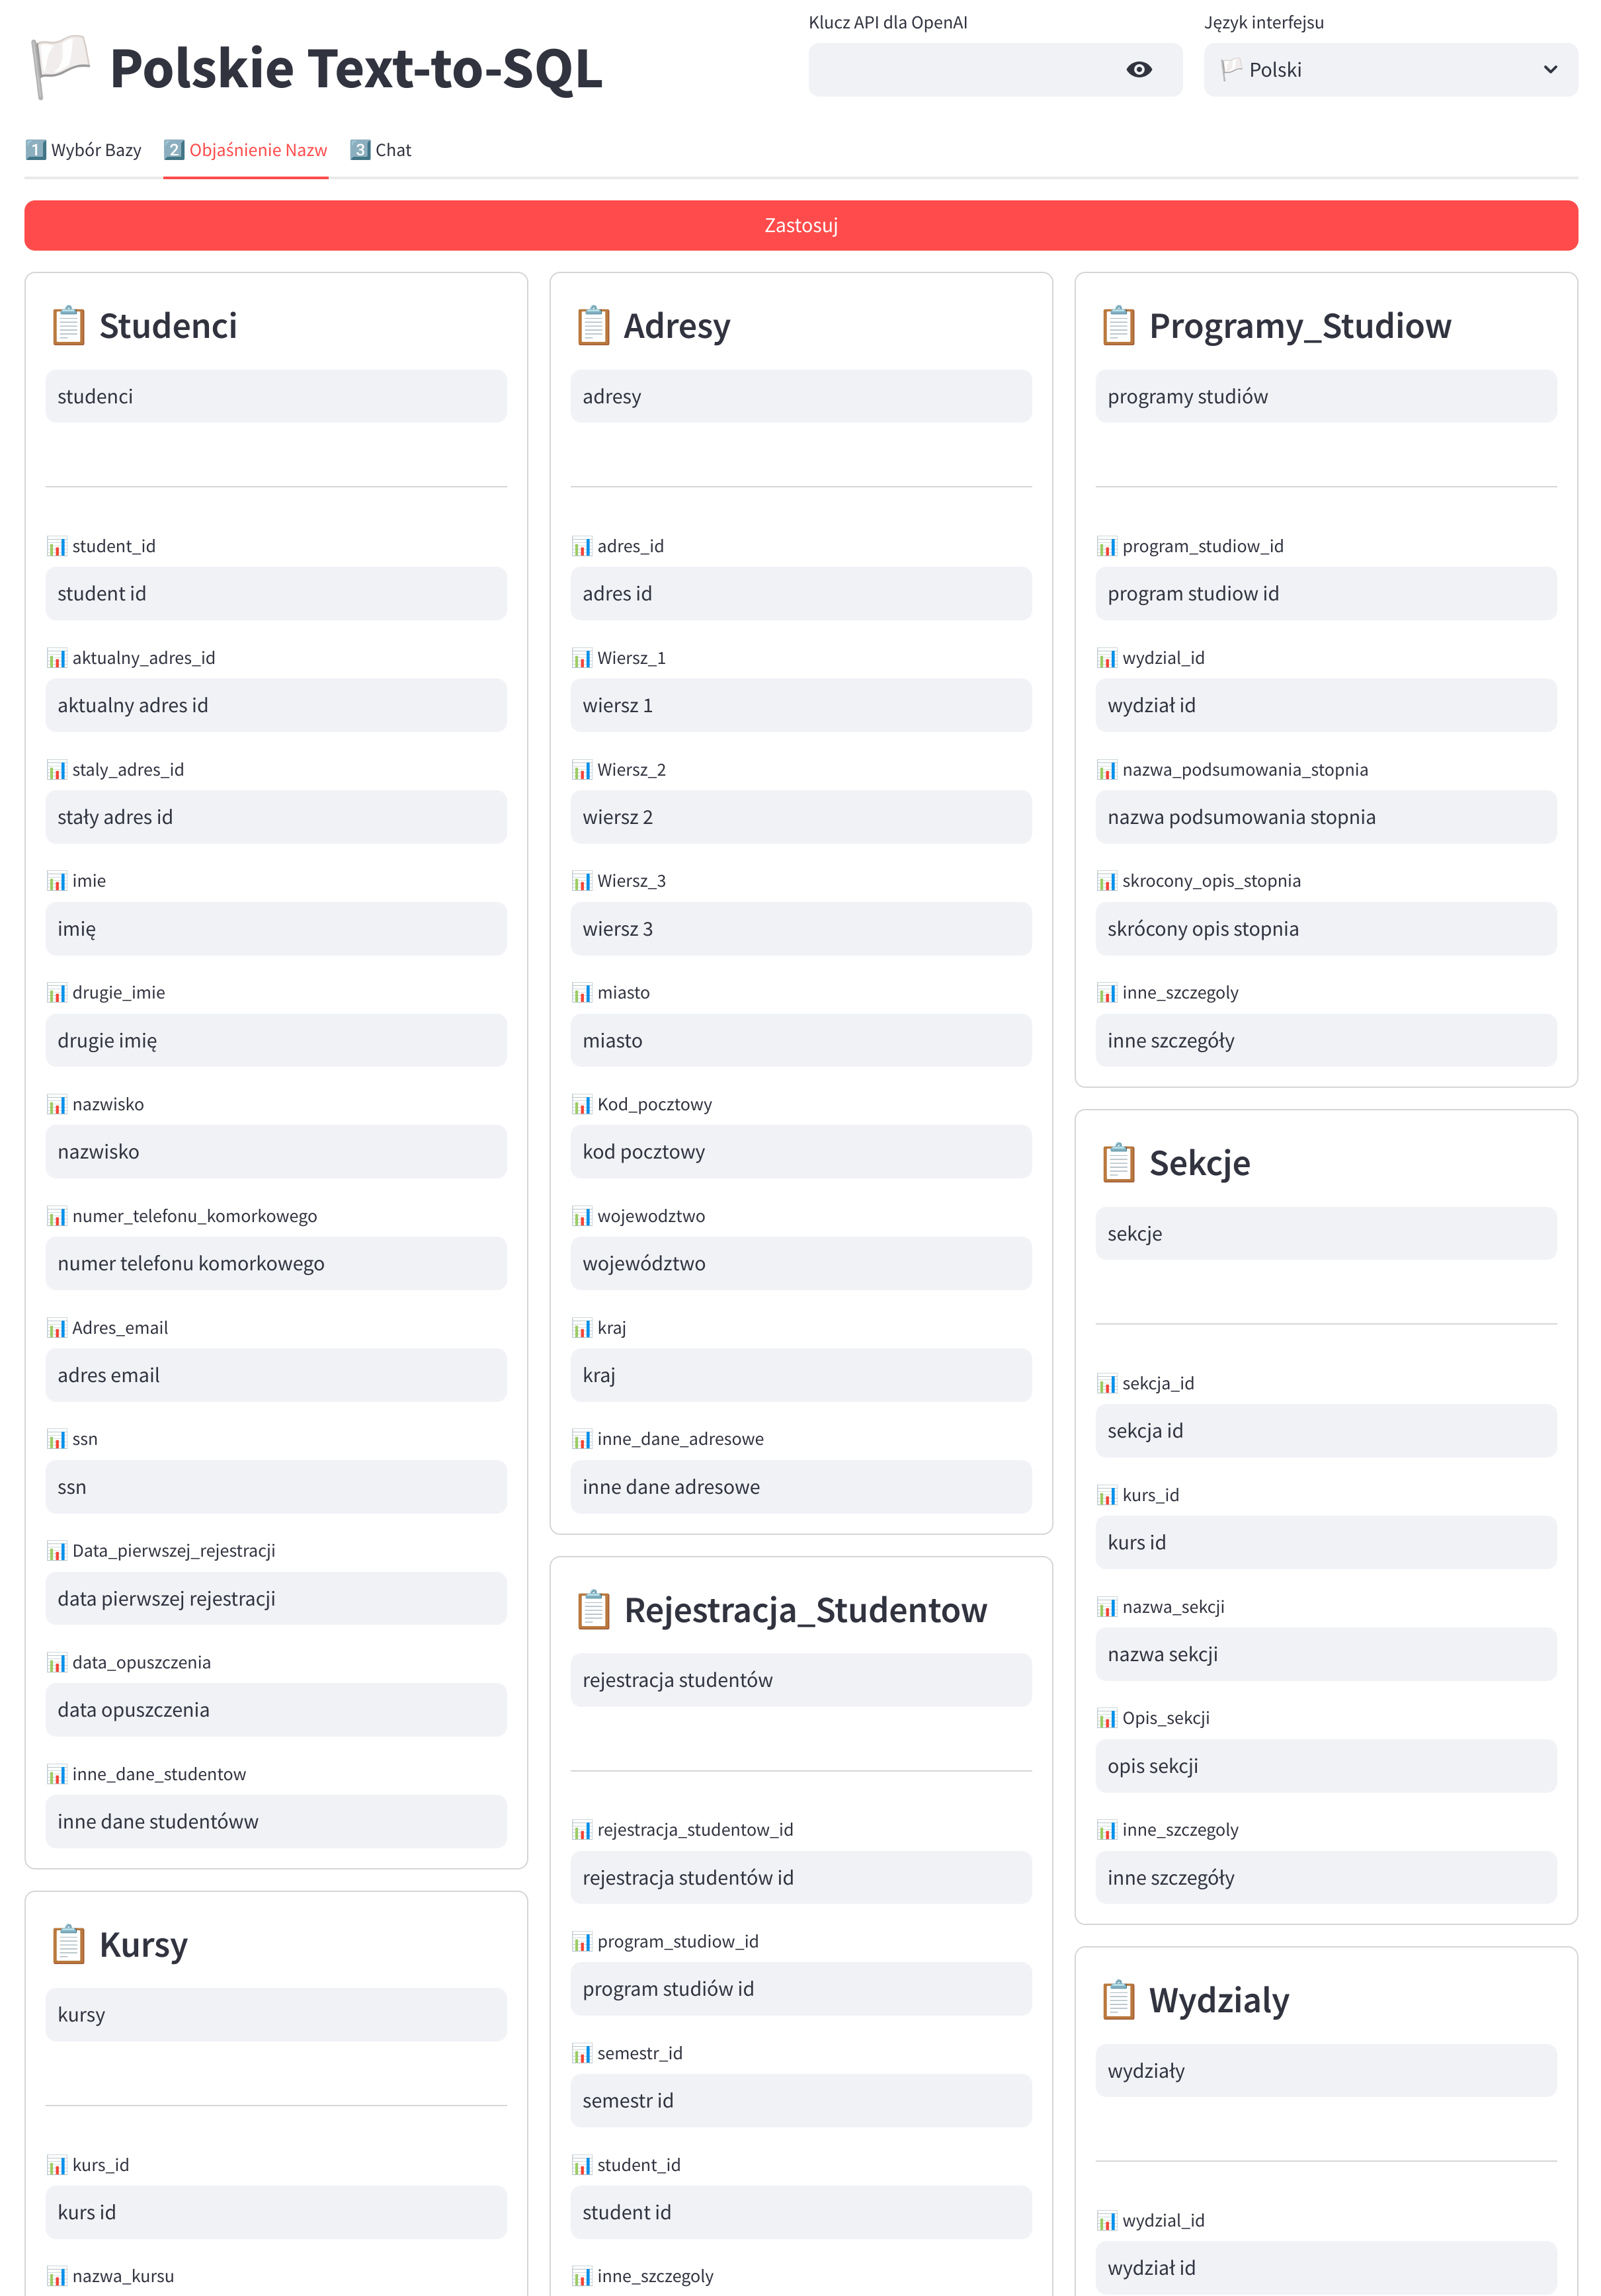
\includegraphics[width=1.0\linewidth]{images/gui_clarification_tab.png}}
  \caption{Zakładka objaśnienia nazw schematu w stworzonym interfejsie graficznym}
  \label{fig:gui-clarification-tab}
\end{figure}

\begin{figure}[ht!]
  \centering
  \fbox{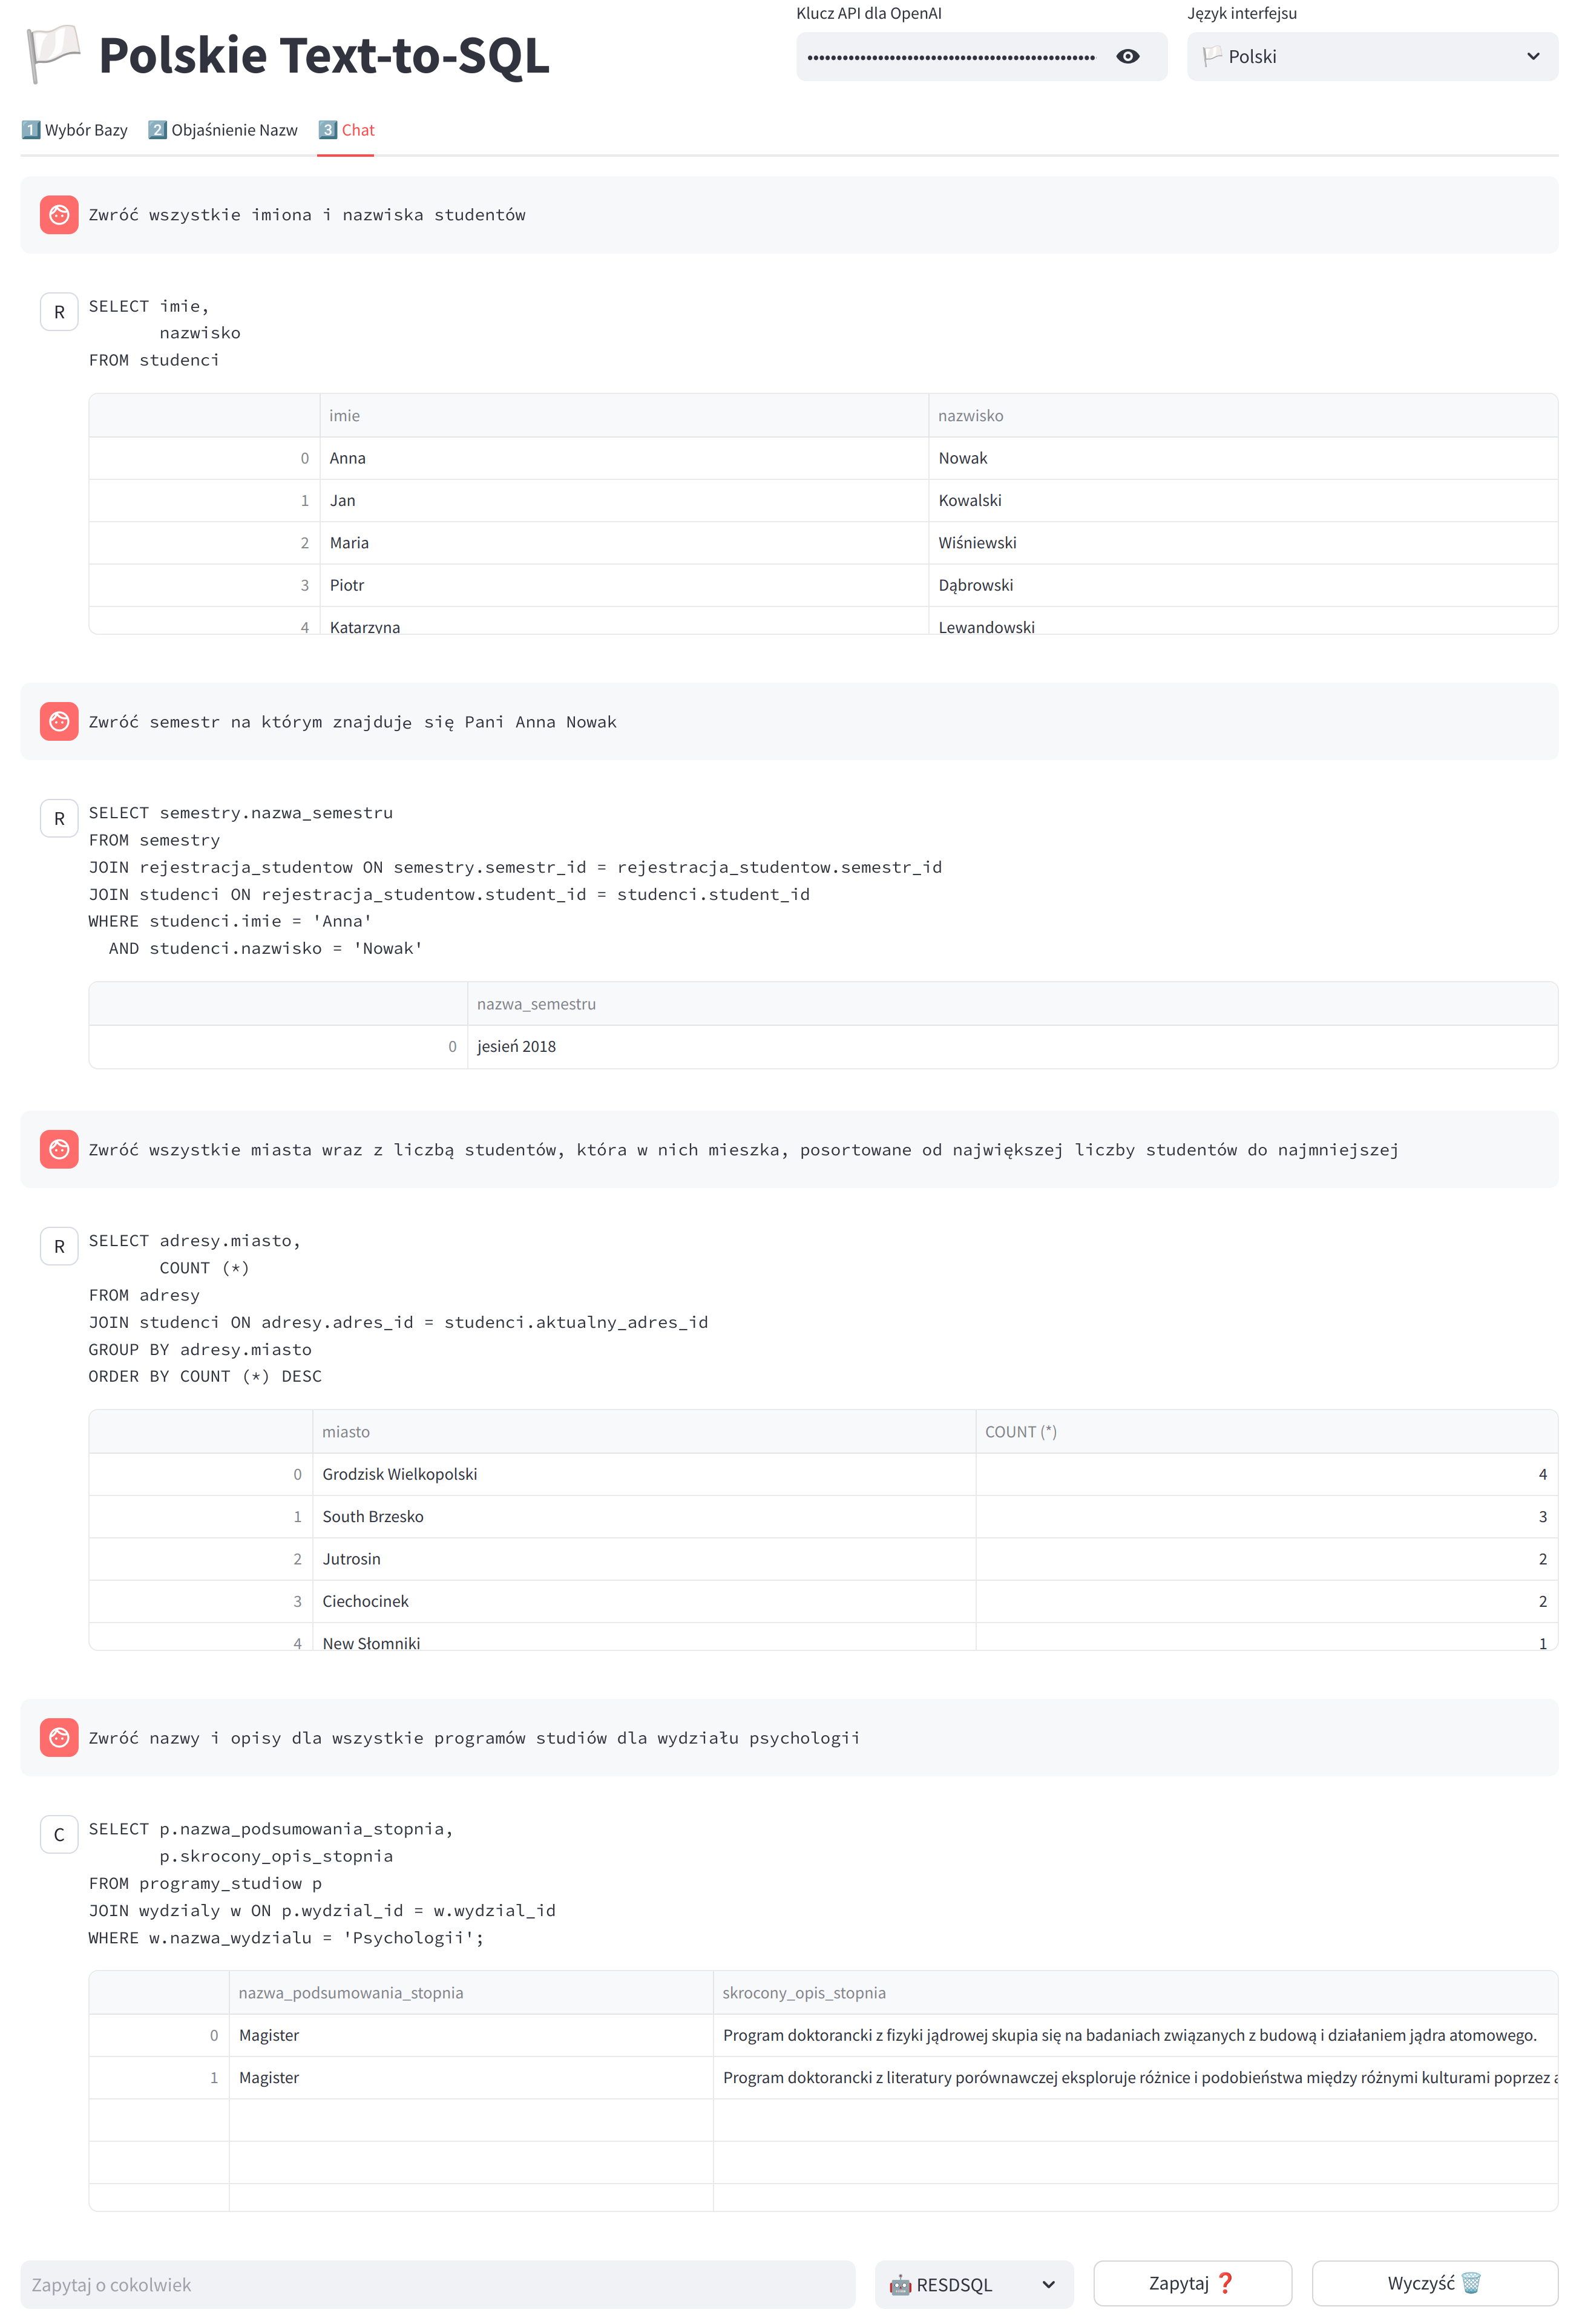
\includegraphics[width=1.0\linewidth]{images/gui_chat_tab.png}}
  \caption{Zakładka chatu w stworzonym interfejsie graficznym}
  \label{fig:gui-chat-tab}
\end{figure}
